\part{Electronic Flight Instruments}

% ==============================================================================
\chapter{Head Down Displays (HDD)}
\label{chap:hdd}

Readouts are color coded. Information will be presented in white when in the normal operating range, yellow for information out of the normal range but not out of limits, and red for out of limit values.

\newpage
\section{Primary Flight Display (PFD)}
\label{sec:pfd}

The \gls{PFD}, \gls{HSI}, ...

\begin{figure}[h]
  \centering
  \colorbox{black}{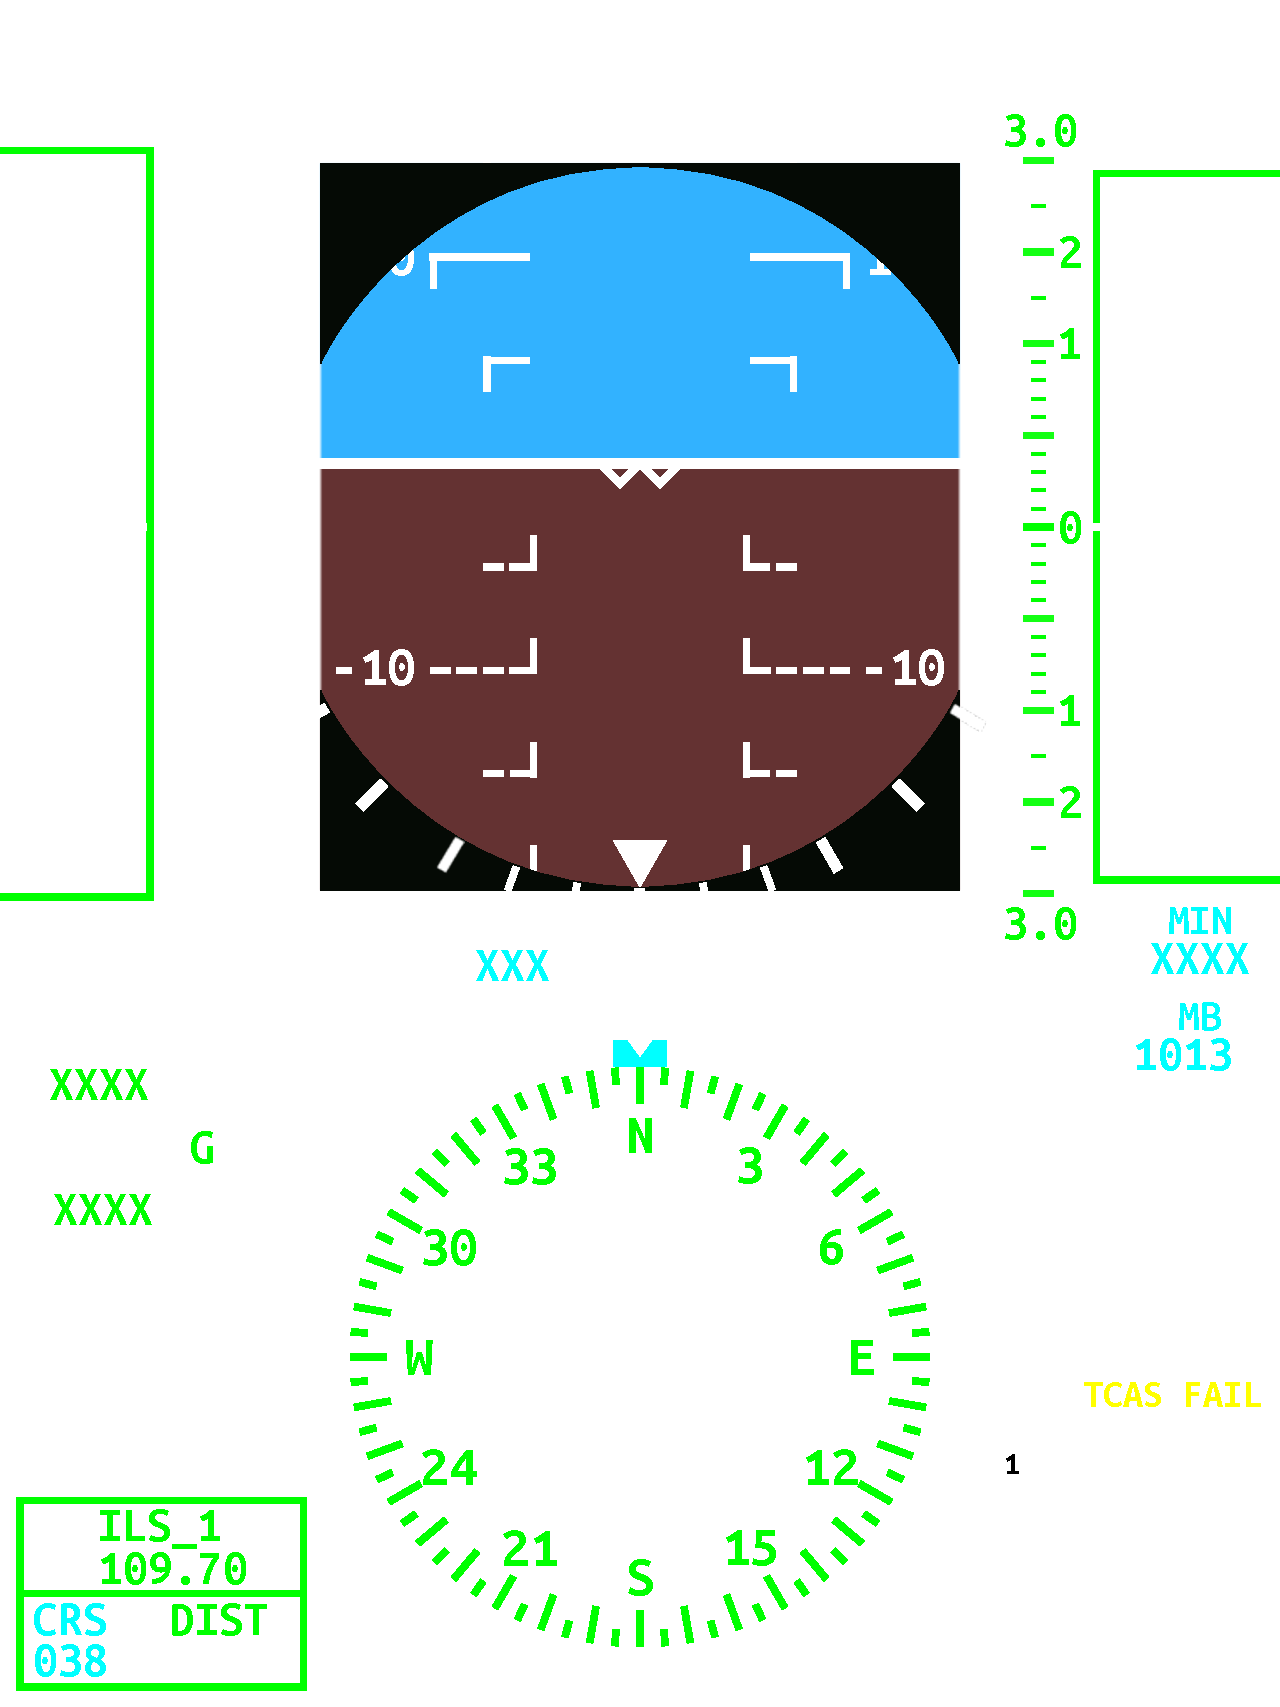
\includegraphics[width=7cm]{figures/hdd/PFD}}
  \caption{Primary Flight Display}
\end{figure}

cyan for VOR/ILS, magenta for FMS

Entered V1 and VR will automatically display on the airspeed indication.

\subsection{Horizontal Situation Indicator (HSI)}
\label{sec:hsi}

Displays Heading, Track, \gls{CDI}, Heading Bug (cyan), Bearing pointers (VOR green, ADF cyan)

\paragraph*{V Speeds}

\begin{itemize}
  \itembf{$V_1$} Critical engine failure recognition speed.
  \itembf{$V_R$} Rotation speed.
  \itembf{$V_H$} Maximum speed in level flight at maximum continuous power.
\end{itemize}

\paragraph*{Autopilot}

\begin{itemize}
  \item left-top (green): HDG, NAV CAPT, (BACK LOC)?
  \item left-bottom (white): NAV ARM

  \item right-top (green): ALT HOLD, GO ARND, GS CAPT, (CAT2)?
  \item right-bottom (white): ALT SEL, GS ARM, (CAT2 ARM)?
\end{itemize}

\newpage
\section{Engine}

\begin{figure}[h]
  \centering
  \colorbox{black}{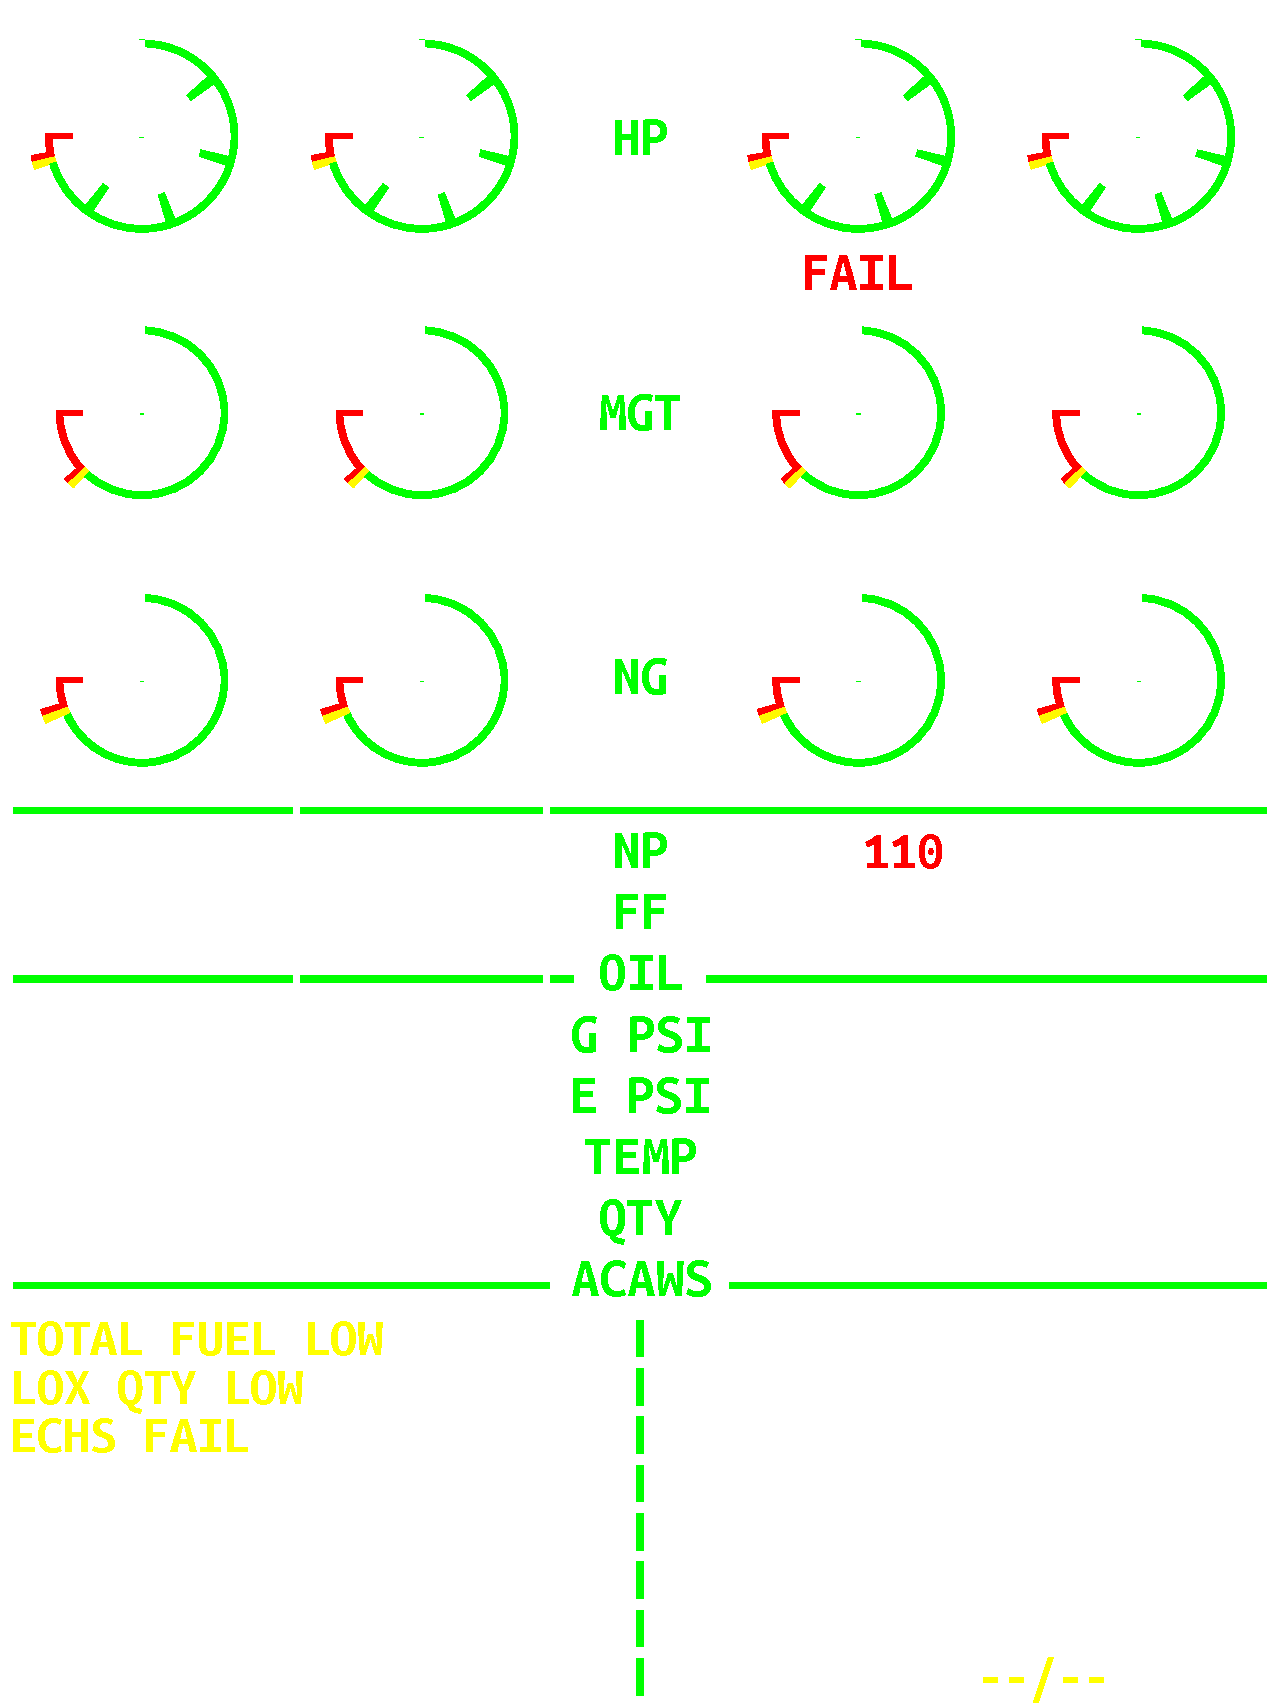
\includegraphics[width=7cm]{figures/hdd/EICAS}}
  \caption{ENGINE and ACAWS display}
\end{figure}

\newpage
\section{CAPS}
\label{sec:caps-airdrop}

\gls{CAPS-airdrop}

\begin{figure}[h]
  \centering
  \colorbox{black}{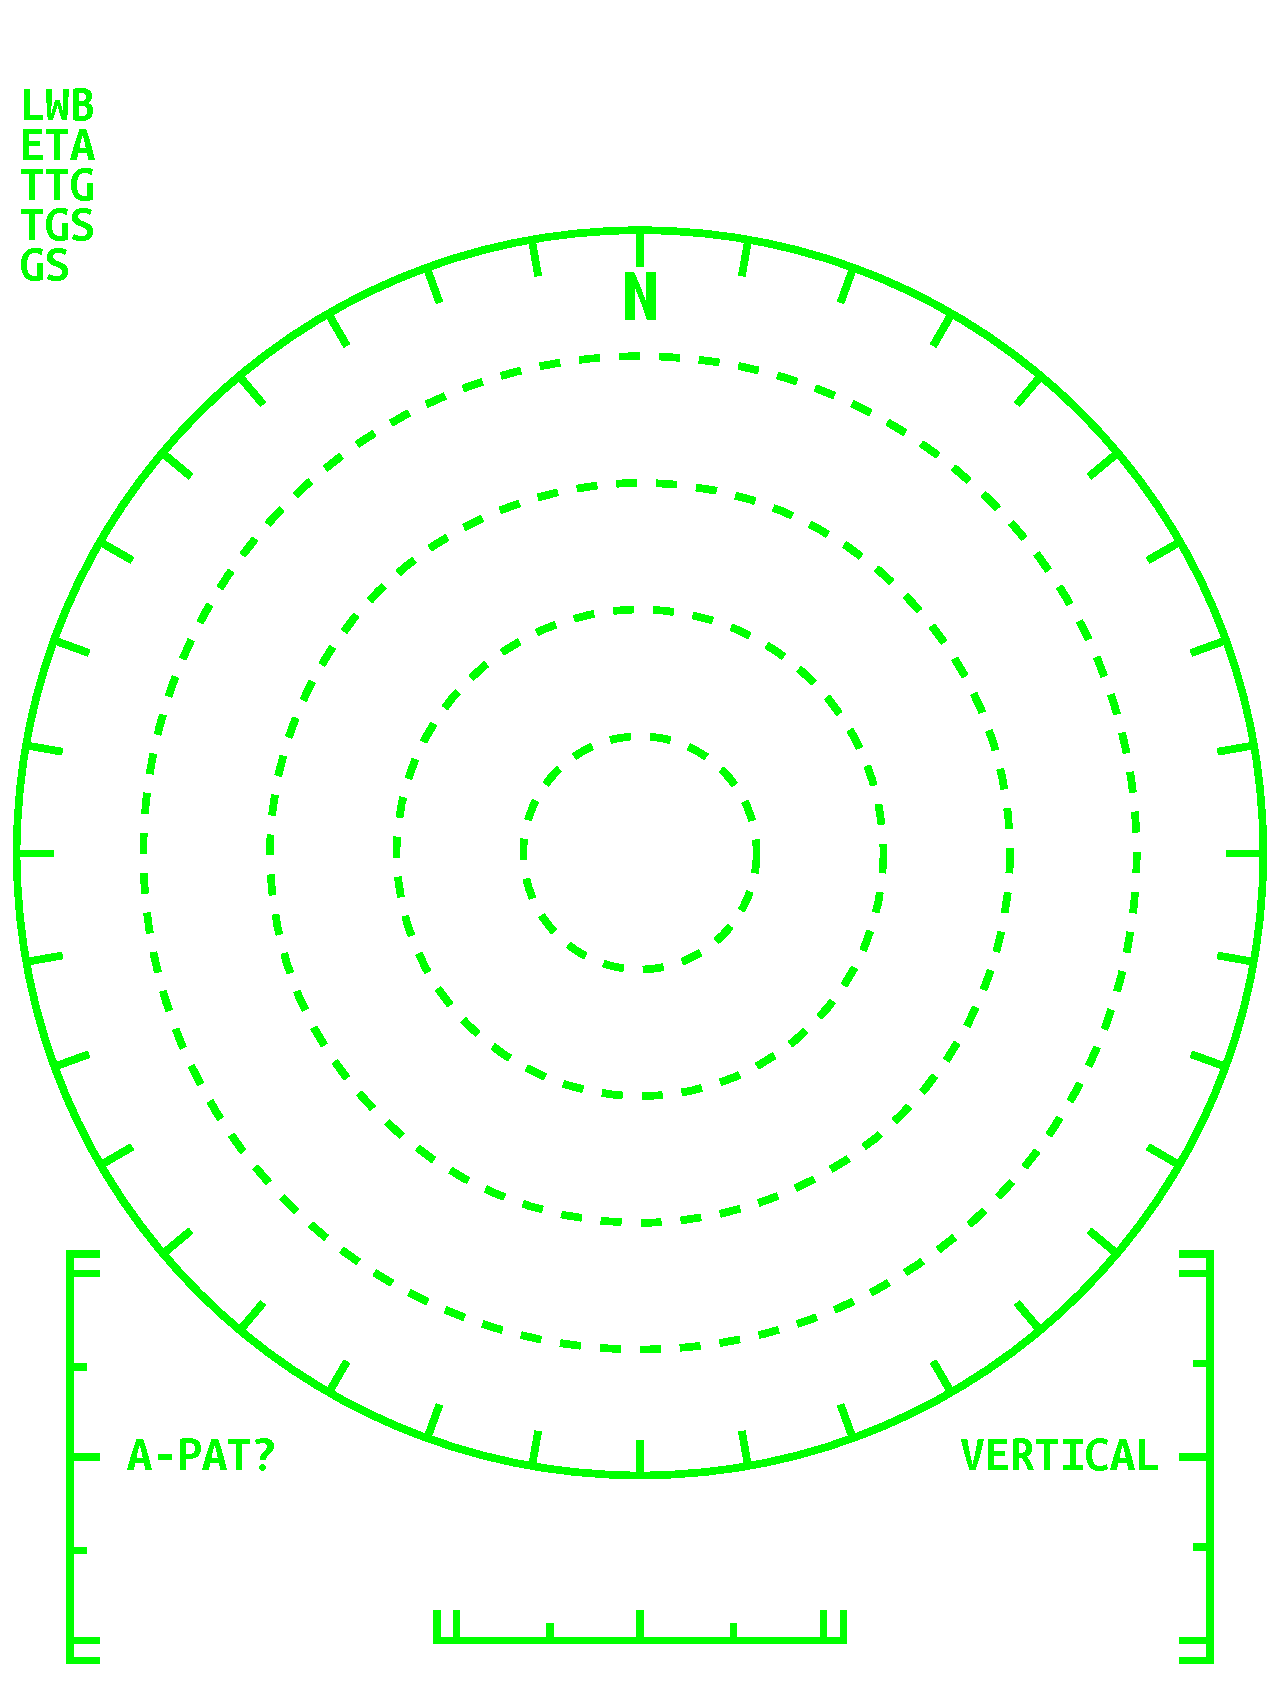
\includegraphics[width=7cm]{figures/hdd/CAPS}}
  \caption{\gls{CAPS-airdrop} display}
\end{figure}

\newpage
\section{System Status}

The SYSTEM STATUS display consists of multiple sections:

\begin{figure}[h]
  \centering
  \colorbox{black}{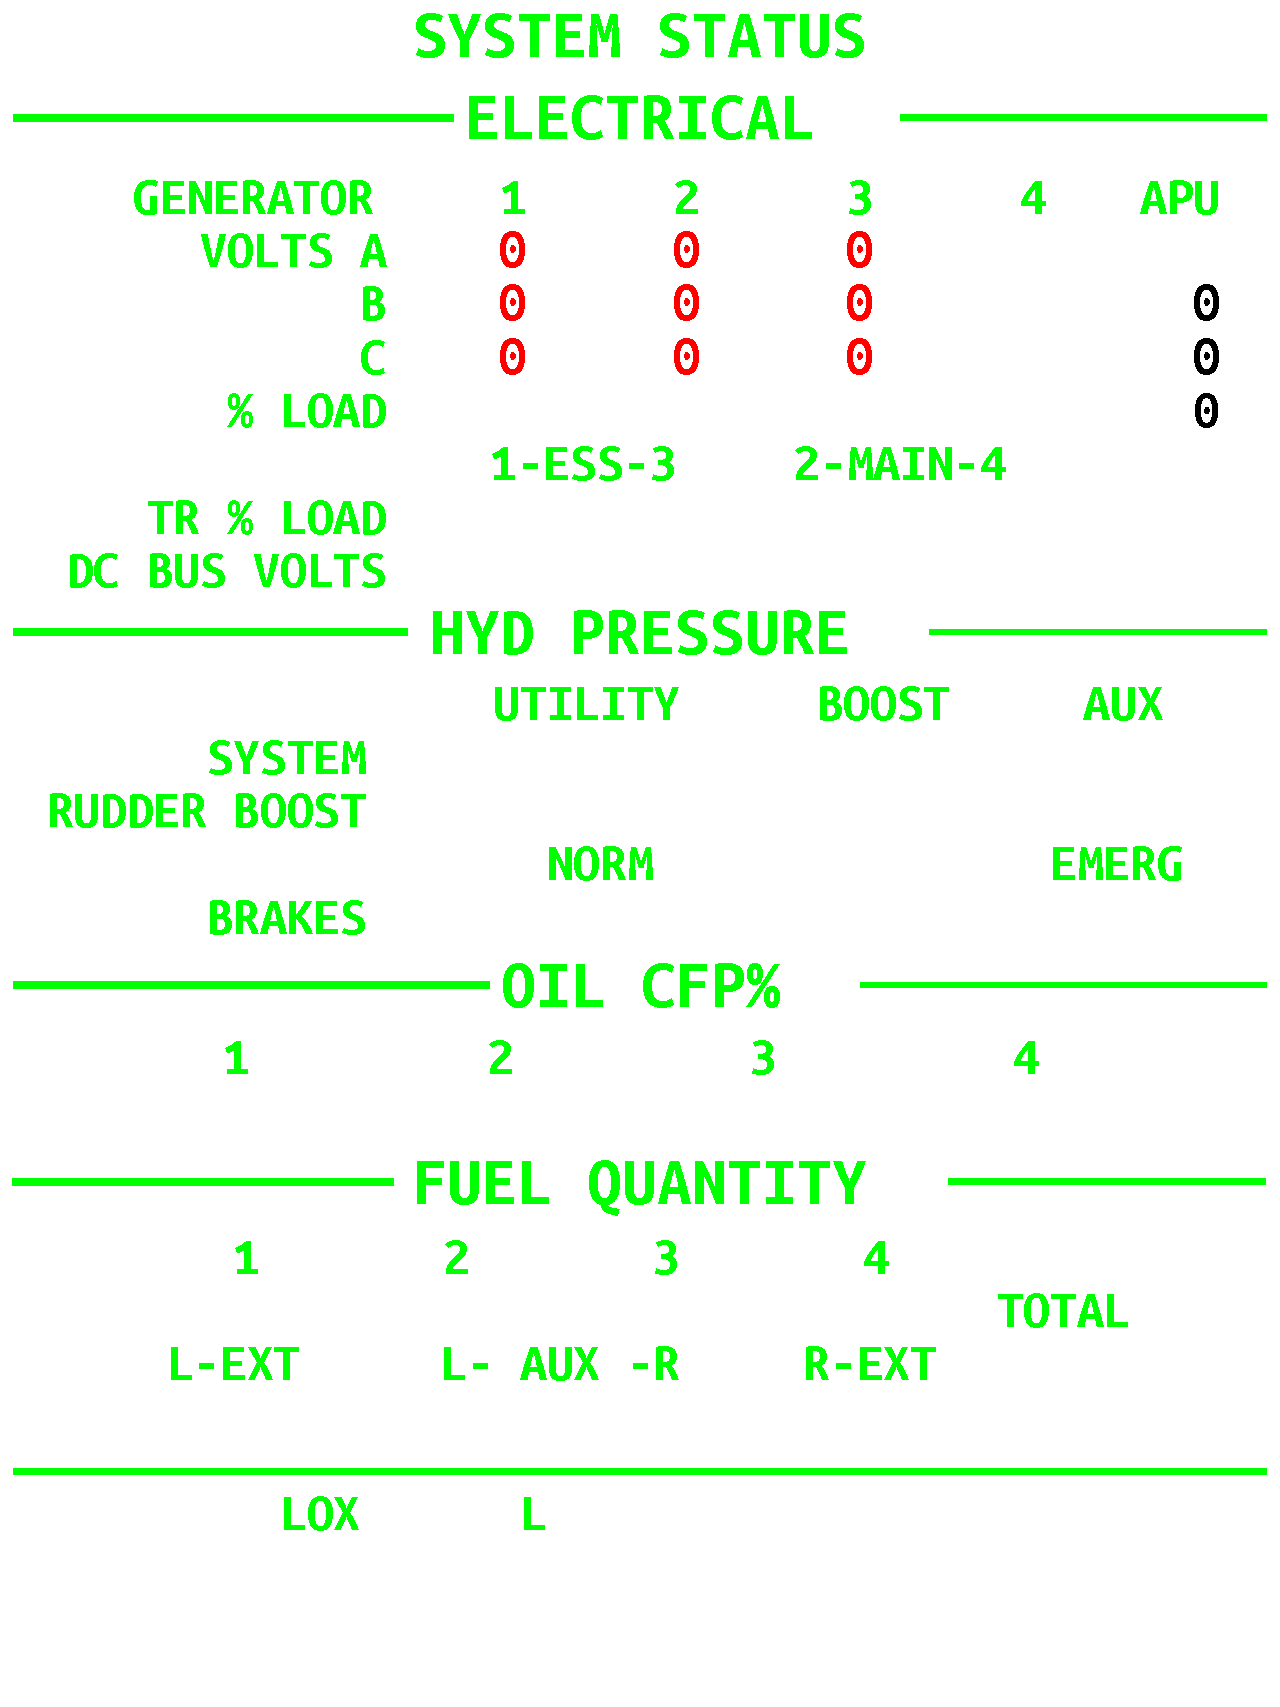
\includegraphics[width=7cm]{figures/hdd/SYSTEM-STATUS}}
  \caption{SYSTEM STATUS display}
\end{figure}

\subsection*{ELECTRICAL}
Generator voltage and percentage of rated current load are shown. Values for generator voltage and load are displayed in columns, labeled from left to right, representing generators 1, 2, 3, 4 and the APU generator. Three voltages are shown in the column for each generator to indicate the voltage of each of the three phases of the generator: A phase, B phase, C phase. Percent of maximum rated load for all five generators (an average of the three phases) is displayed in the row below the C phase voltage. If the system is not powered, OFF will be displayed in the appropriate data blocks. If the system is disconnected (eg. EXT PWR/OFF/APU not APU for APU), three dashed lines will be displayed. The display symbols are generated by the multifunction display units based on information received from the mission computer. 

\subsection*{HYD PRESSURE}

\subsection*{OIL CFP\%}

\subsection*{FUEL QUANTITY}

% ==============================================================================
\chapter{AMU}
\label{chap:amu}

The \gls{AMU}, \gls{CNBP}, \gls{CMDU}, \gls{CMDS}, \gls{CADC}
